\chapter{Marco Teórico}

 En este capitulo se aborda el marco teórico necesario para comprender más fácilmente el desarrollo de los capítulos posteriores. Se analiza el problema del tráfico en general, los simuladores y la teoría detrás del algoritmo a utilizar.

\section{Problema del tránsito vehicular}

En gran parte del mundo se está produciendo un crecimiento sostenido del parque automotor lo que ocasiona una serie de problemas que afectan la calidad de vida de las personas relacionados con el agravamiento de las congestiones vehiculares \citep{Cepal2003}.

Este problema tiene un gran impacto en el desarrollo de las ciudades por lo que es un componente principal en los planes estratégicos para su crecimiento.

La congestión ocasiona una progresiva merma en la velocidad promedio de circulación, lo que incrementa la duración de los viajes, aumenta el consumo de combustible y la contaminación atmosférica y sonora, lo que repercute directamente en la salud de las personas. 
además se genera una exigencia en las vías de tránsito que ocasiona un deterioro mayor de calles y rutas.

Uruguay no escapa a este fenómeno en particular Montevideo, donde el aumento del parque automotor está en ascenso constante desde el 2005 \citep{INE2014} 
Y según proyecciones el crecimiento seguiría en un promedio de 4.5\% anual hasta el 2020. \citep{BBVA2013}

Esto viene de la mano con el sostenido aumento de las ventas de vehículos  desde el 2003 \citep{Autoanuario2014}

Los expertos indican que la congestión ya está instalada y la infraestructura vial no acompasó este crecimiento. además se indica que Montevideo es la ciudad con más semáforos por automóvil en Latinoamérica. Con más de 620 cruces semaforizados, alguno de los cuales no están coordinados.\citep{Subrayado2013}

Esto lleva a las autoridades a buscar nuevas soluciones, en el caso de Montevideo se trata del plan de movilidad urbana \citep{PlanMovilidad} que tiene como objetivo mejorar la eficiencia del transporte publico y democratizar el acceso al mismo. Uno de sus puntos principales es el desarrollo de corredores de tránsito para mejorar la movilidad. En la siguiente sección se darán detalles sobre corredores y en particular el Corredor de Garzón.

\section{Corredor Garzón}
COMPLETAR
Estas referencias son las que usamos en el paper:
\citep{olivera2013}
\citep{olivera2015}	


\subsection{Descripción del corredor de Garzon}	
El corredor Garzón esta localizado al Nordeste de Montevideo Uruguay, fue construido como parte de un plan de movilidad que incluye otros 4 corredores de la ciudad. Tomando en cuenta de un extremo al otro conecta Colon con Paso Molino y teniendo 6.5km de largo, atraviesa muchas calles importantes como Millan p.e. que lleva a una autopista (Ruta 5). Es importante aclarar que no es solo una conexión de extremo a extremo ya que barrios como Sayago y otros constan de una gran cantidad de habitantes.
El Corredor consiste básicamente en 3 calles paralelas e independientes; donde 2 de ellas son de dos carriles de una sola mano y entre medio de estas esta una calle doble vía con un carril para cada vía que es exclusivamente usado por ómnibus.

\subsection{¿Es el Corredor de Garzon un BRT?}
Bus Rapid Transit (BRT) es una solución innovadora, de alta capacidad y de menor costo para el transporte público que puede alcanzar el rendimiento y los beneficios de modos ferroviarios con un costo significativamente menor. Se trata de un sistema integrado de transporte basado en autobuses para el transporte de los pasajeros a sus destinos de manera rápida y eficiente. Al mismo tiempo ofrece la flexibilidad necesaria para satisfacer una variedad de condiciones locales. Los elementos del sistema de BRT pueden ser fácilmente personalizados a las necesidades de la comunidad e incorporan tecnologías de última generación de bajo costo que atraen a más pasajeros y en última instancia ayudan a reducir la congestión de tráfico en general.

Un BRT contiene características similares a un tren ligero o el sistema de metro por ese motivo es mucho más confiable, conveniente y más rápido que los servicios regulares de autobús. Con las características adecuadas, el BRT es capaz de evitar las causas de los retrasos que suelen tener los servicios regulares de autobús, como estar atrapado en el tráfico y hacer cola para pagar a bordo.

Un corredor de BRT es un tramo de carretera o caminos contiguos donde hay un carril exclusivo para una linea de autobús o varias líneas de autobuses con una longitud mínima de 3 kilómetros (1,9 millas) que ha dedicado los carriles bus. El Estándar BRT se va a aplicar a los corredores de BRT específicos en lugar de a un sistema de BRT como un todo (en el caso de montevideo el BRT como un todo seria el STM), porque la calidad de cada BRT en ciudades con múltiples corredores puede variar significativamente *.

Para considerarse BRT, un corredor debe:

ser al menos 3 kilometros de longitud con carriles exclusivos,
Llegar a  4 o más puntos en específico elemento derecho de vía,
Llegar a 4 o más puntos en elemento de alineación electroducto; y
Llegar a 20 o más puntos en los cinco elementos Basicos de un BRT.


SEMÁFOROS. Un corredor debe de funcionar al igual que una autopista en el sentido de que una vez que se entra debería ser posible mantener la velocidad máxima sin tener que parar seguido por lo que no deberían de haber semáforos cerca uno del otro, de haberlos la sincronización será la clave para minimizar los tiempos de espera.
CALLES PARALELAS. Tener calles paralelas es de vital importancia para un corredor ya que una de las formas de minimizar los tiempos de espera es prohibir los giros a la izquierda, y una calle paralela provee la facilidad de poder realizarlo sin estorbar en el corredor.
LINEAS DE ÓMNIBUS. Los corredores son realizados para mejorar tramos largos donde viaja unicamente una línea sola de transporte urbano.
GIRO A LA DERECHA CON LUZ ROJA. Actualmente en muchos países se encuentra reglamentada una ley que permite a los conductores doblar a la derecha con luz roja ya que la misma (a menos que se especifique) es tomada como un cartel de Pare SOLAMENTE para doblar a la derecha. Esta ley acorta los tiempos de luz verde de las transversales mejorando así la velocidad promedio en el corredor.

Presenta un carril exclusivo para ómnibus y preferenciales
http://www.montevideo.gub.uy/ciudadania/stm-transporte-metropolitano/plan-de-movilidad/corredores

Tiene 6km de largo , extendiéndose desde ...  hasta ..
%http://www.montevideo.gub.uy/sites/default/files/articulo/corredor_garzon.pdf

Agregar mapa y poner referencia de donde se saco

Los problemas de sincronización de semáforos fueron admitidos en varias publicaciones.

18 diciembre 2013 - Corredor Garzón lucha contra el tiempo %http://www.elpais.com.uy/informacion/imm-corredor-garzon-tiempos-cambios.html
Dice que antes de Garzon se demoraba promedio 18 minutos, y al inaugurar el corredor 30 minutos. Después se mejoro algo para equilibrar los tiempos
Para el jerarca, eso se dio "con la diferencia de que hoy hay 15 semáforos más y se ganó en seguridad". En concreto, tras la obra, se pasó de tener 5 semáforos a 20. Según Campal, su des-coordinación inicial, entre otros aspectos, fue lo que provocó tales demoras, generando malestar en los usuarios.
inversión de 60 millones


4 agosto 2013 - Garzon desde un omnibus %http://www.elpais.com.uy/informacion/corredor-garzon-visto-bus.html


30 julio 2013  - Intendetnta admite errores %http://www.elpais.com.uy/informacion/garzon-olivera-admitio-errores.html
La intendenta admte errores y dice: no se ha logrado sincronizar los semáforos. Hay un tema con el software,(y) la empresa subcontratada no ha dado los resultados esperados


Abril 2013 - Otro Corredor con obras paralizadas por criticas a GArzon
%http://www.elpais.com.uy/informacion/marcha-atras-en-corredor-agraciada.html


\section{Sincronización de semáforos}
--Esto va en Garzon, cuando decimos que tiene problemas:
Por todo esto es relevante el tema de la sincronización de semáforos para agilizar el tránsito y no generar congestiones, aumentando la velocidad promedio de los viajes y mejorando las perspectivas de desarrollo de la ciudad así como la calidad de vida de sus habitantes.


Un buen funcionamiento de los semáforos es fundamental para asegurar que el trafico se mueva con eficiencia y a la vez aporte seguridad a los peatones. 
Existen diversos métodos para lograr la coordinación necesaria que van desde simples mecanismos de reloj a sistemas computarizados que se ajustan en tiempo real con ayuda de sensores en la calle.

Cabe destacar que cuanto mayor cantidad de semáforos para sincronizar mayor es la dificultad a la hora de encontrar una solución eficiente. Por este motivo se considera a este prolijea como NP-Dificil, es decir que no existe hasta el momento un método determinístico que lo resuelva.


Existen diversas métodos para solucionar este problema, uno de los mas desarrollados y efectivos son los algoritmos evolutivos los cuales son usados en este trabajo y serán explicados a continuación.

\section{Algoritmos Evolutivos}

Uno de los puntos importantes del presente trabajo son los algoritmos genéticos por lo que se dedica esta sección para  brindar un repaso por los conceptos y definiciones necesarias para comprender el desarrollo posterior de la solución.

Los algoritmos evolutivos son métodos no determinísticos que se inspiran en la evolución natural de las especies utilizando conceptos como población, cruzamiento, mutación, selección, etc. Estos se utilizan para resolver problemas de optimización y búsqueda, entre otros \citep{Nesmachnow2002}.

Es una técnica iterativa que busca en cada paso mejorar las soluciones por medio de operadores basado en un criterio predefinido para maximizar o minimizar.

Este tipo de solución ha demostrado su utilidad en una amplia variedad de problemas complejos.


\subsection{Algoritmos Genéticos}
El algoritmo genético es uno de los más populares dentro de los algoritmos evolutivos.

La idea base es que partiendo de una población inicial de individuos se seleccionan los mejores en base a su aptitud respecto a solucionar el problema y estos se utilizan para generar nuevos individuos ya sea por combinación o modificación. Por tanto en cada paso obtenemos mejores soluciones hasta detenernos usando un criterio de parada ya sea el número de iteraciones o cuando ya no se puede mejorar más la solución.

Un individuo es una codificación de la solución que resuelve el problema.
La población inicial puede generarse aleatoriamente o basándose en algún conocimiento previo.
La función de evaluación indica que tan buena o apta es una solución en comparación con las demás.
En cada iteración la cual se llama generación se aplican operadores de cruzamiento estos son formas de combinar a los individuos para obtener otros que potencialmente sean una mejor solución y también cambios aleatorios sobre los individuos llamado mutación.

Por tanto se van seleccionando, combinando y cambiando las mejores soluciones en un proceso que va obteniendo mejores soluciones.
El criterio de parada nos indica cuando termina este proceso, ya sea por que se alcanzó un número de generaciones predefinidos o por que la mejora no es evidente. Al final se devuelve la mejor solución encontrada en todo el proceso.

Hay que indicar que no es una técnica exacta pero si logra muy buenas aproximaciones y es muy buena en problemas complejos por su flexibilidad y robustez. 


\subsubsection{Representación de soluciones}
No podemos trabajar directamente sobre las soluciones, por lo que tenemos que codificarlas en un modelo que nos sirva para poder aplicar el algoritmo.
La inspiración biológica se ve en los nombres que adopta esta representación, llamada Cromosoma que es un vector de genes y cada valor de un gen se llama alelo.
En general se codifica un vector de números binarios o reales de largo fijo, lo que facilita la aplicación de los operadores.

\subsubsection{Función de Evaluación} 
Indica que tan bueno es un individuo para resolver el problema en cuestión con un valor conocido como Fitness. Este se utiliza para seleccionar a los mejores y de esta forma guiar la exploración hacia la mejor solución.
Se deben tener en cuenta las restricciones del problema para que las soluciones no factibles no sobrevivan.
En general es donde se consume el mayor tiempo del algoritmo en comparación con los demás operadores.

\subsubsection{Operador de Selección}
Existen diversos operadores de selección , su función es que las mejores características de los individuos se mantengan en las siguientes generaciones.
Los tipos más populares son:

\begin{itemize}
	\item Ruleta: También conocida como selección proporcional elige aleatoriamente individuos en la cual la probabilidad de selección es proporcional al valor de fitness.
	\item Torneo: Se elige aleatoriamente un determinado número de individuos los cuales compiten entre si.
	\item Elitismo: Los mejores individuos son mantenidos entre las generaciones.
\end{itemize}

\subsubsection{Cruzamiento}
Su función es combinar individuos para lograr mejores soluciones. 
Existe una tasa que se puede modificar para indicar la probabilidad de que se realice el cruzamiento.

\begin{itemize}
	\item Cruzamiento de un punto: A partir de dos padres se selecciona un punto al azar de los cromosomas obteniendo dos trozos que se combinan para obtener dos hijos. Se explica en la figura ~\ref{fig:cruzamiento1}
	\item Cruzamiento multipunto: El método anterior se puede generalizar para obtener más puntos de corte y más recombinaciones.
\end{itemize}

\begin{figure}[h]
	\centering
	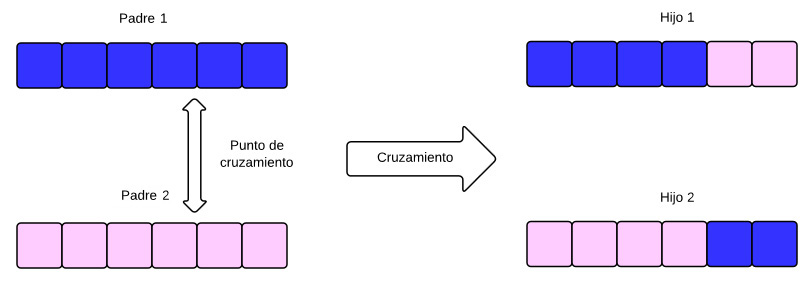
\includegraphics[width=\textwidth]{Figures/cruzamiento1}
	\caption{Cruzamiento de un punto}
	\label{fig:cruzamiento1}
\end{figure}

\subsubsection{Mutación} 
Indica el método utilizado para modificar un individuo, esto se realiza para lograr más diversidad y no caer en máximos locales. En general aplica una modificación aleatoria en el cromosoma.También hay una tasa de probabilidad, en general es baja. En el caso de un cromosoma binario se aplica la inversión sobre un alelo.

\begin{figure}[h]
	\centering
	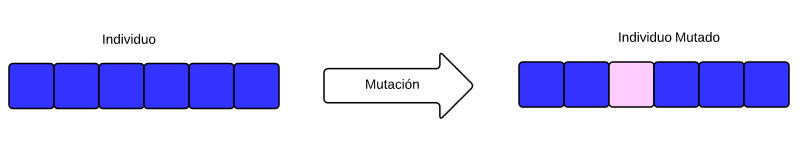
\includegraphics[width=1\linewidth]{Figures/mutacion1}
	\caption{Mutacion por inversión binaria}
	\label{fig:mutacion1}
\end{figure}


\subsubsection{Reemplazo} 
Se indica cual es el criterio que debemos tomar para generar una nueva población, ya sea tomando solo los hijos creados o comparando también con los padres o aplicando algún otro criterio.

\subsubsection{Criterio de parada} 
Indica cuando debe terminar el algoritmo, puede ser definiendo un número fijo de generaciones o analizando si el mejor valor de fitness se mantiene relativamente constante durante un número determinado de generaciones.

\subsection{Funcionamiento}

El esquema básico de funcionamiento es el siguiente:


\begin{algorithm}%[!ht]
	\caption{Algoritmo Genético}
	\label{alg:algoritmo_genetico_simple}
	\begin{algorithmic} [1] 
		{
			%\small
			\STATE {Inicializo( Pob(0))}
			\STATE \texttt{generacion} = 0
			\WHILE {\text{No llegue al criterio de parada}}
			\STATE {Evaluar Pob(generacion)}
			\STATE {Padres = Seleccionar(Pob(generacion))}
			\STATE {Hijos = Cruzamiento(Padres) y Mutacion(Padres)}
			\STATE {NuevaPob = Reemplazar Pob(generacion) con Hijos}
			\STATE \texttt{generacion}++
			\ENDWHILE
			\RETURN Mejor solución
		}
	\end{algorithmic}
\end{algorithm}



% ctrl+t comenta
%\begin{algorithm}%[!ht]
%	\caption{Genetic Algorithm}
%
%	\begin{algorithmic} [1] 
%		{
%
%			\STATE {Init( Pop(0))}
%			\STATE \texttt{generation} = 0
%			\WHILE {\text{NOT Stop Criteria}}
%			\STATE {Evaluate Pop(generation)}
%			\STATE {Parents = Selection(Pop(generation))}
%			\STATE {Children = Crossover(Parents) and Mutation(Parents)}
%			\STATE {NewPop = Replace Pop(generation) with Children}
%			\STATE \texttt{generation}++
%			\ENDWHILE
%			\RETURN Best solution
%		}
%	\end{algorithmic}
%\end{algorithm}


\subsection{Algoritmos genético multiobjetivo}

En este caso se busca una solución que satisfaga de forma simultánea tanto las restricciones del problema como varios objetivos distintos.



\subsection{Algoritmo Genético Paralelo}
Los problemas complejos suelen requerir una alta demanda computacional por lo que aplicar técnicas de paralelización es útil para lograr tiempos de ejecución menores.

Existen varios niveles de paralelización ya sea a nivel global enfocándonos en paralizar la función fitness, a nivel de la población, o a nivel del individuo. \citep{Nesmachnow2002}

En el caso de los algoritmos genéticos gran parte del tiempo se ocupa en la etapa de evaluación, por esta razón es un buen método para distribuir la carga en varios procesadores para que las evaluaciones se realicen en paralelo.


\subsection{Maestro-Esclavo}

En este modelo un proceso maestro es el encargado de realizar los operadores básicos del algoritmo y distribuir a procesos esclavos la evaluación de la función fitness para un conjunto de individuos, el esclavo devuelven el resultado y luego el maestro es el encargado de continuar ejecutando los operadores.

De este modo aumenta la eficiencia computacional del algoritmo ya que una de las funciones más costosas es distribuida entre varios nodos.

\begin{figure}[H]
	\centering
	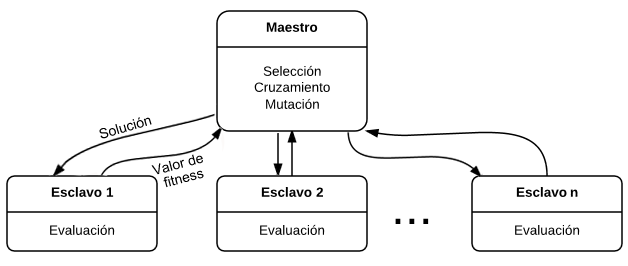
\includegraphics[width=0.7\linewidth]{Figures/diagrama-master-slave}
	\caption[Modelo Maestro-Esclavo]{Modelo Maestro-Esclavo}
	\label{fig:diagrama-master-slave}
\end{figure}

\subsection{Resumen}
Los algoritmos evolutivos han demostrado su eficiencia en la resolución de gran cantidad de problemas de optimización. Si nos enfocamos en la resolución del problema de sincronización de semáforos existen algunas opciones para ayudar en su resolución, entre las que se encuentra la simulación microscópica o macroscópica del tráfico los cuales serán explicados en la siguiente sección.


\section{Simulación}

\subsection{Simuladores de tráfico}
Los simuladores de tráfico son programas que simulan el movimiento de vehículos sobre una red de calles, es una herramienta muy usada en la investigación de tráfico vehicular; así como estudio de congestiones o análisis de impacto que tendrán nuevas infraestructuras.  Las razones para usar una simulación son varias, entre ellas se encuentra  la rapidez, ya que la simulación se puede realizar en tiempo mucho más rápidos que en la realidad, el costo en dinero pues no estamos afectando el escenario real  y tampoco tenemos que modificar o detener el escenario real para probar nuevos parámetros. además nos sirve para poder prever situaciones que podrían darse bajo determinadas circunstancias.

Los simuladores se pueden dividir en microscópicos o macroscópicos según el nivel de detalle de la simulación. Un simulador macroscópico modela  el tráfico vehicular como un fluido. En cambio un simulador microscópico simula el movimiento de cada vehículo según sus características particulares.

SUMO\citep{SUMO} es uno de los simuladores abiertos más populares, es microscópico y utiliza una serie de archivos  XML que representan las rutas, los vehículos y el tráfico.  

Cuanto más crece el número de vehículos y la complejidad de la red de mapas más difícil se hace crear la entrada básica que necesita el simulador. Aunque existen diversas herramientas que ayudan a este proceso aún se requiere un trabajo manual para el acondicionado de estos archivos.

En las siguientes secciones se muestra más en detalle algunas de sus funcionalidades y características.





\section{Trabajos relacionados}

La investigación del estado del arte se realizo con dos objetivos en mente, el primero analizar las distintas soluciones que existen actualmente para el problema y segundo encontrar nuevas prácticas, algoritmos o utilidades que pudieran fortalecer la solución.

El problema del tráfico optimizando las luces de los semáforos se puede resolver por muchos métodos como  redes neuronales \citep{Lopez1999}, lógica difusa \citep{Lim2001}, redes de petri \citep{DiFebbraro2002}, etc; por lo tanto la cantidad de soluciones encontradas fue abundante y variada por esto se decidió enfocarse en soluciones lo más cercanas a la propuesta y en otras que tuvieran alguna particularidad interesante para destacar.


\begin{itemize}
	\begin{item}
		\bibentry{Sanchez2004}
		
		Este trabajo se basa en tres puntos: El uso de algoritmos genéticos para la optimización , simulación de autómatas celulares para la función de evaluación del tráfico, y un cluster para realizar ejecuciones en paralelo.
		El modelo es pequeño con 5 calles de 2 vías que se intersectan.
		La codificación del cromosoma es una tira de números enteros, donde se codifica para cada intersección cual calle está habilitada en cada ciclo.
		Usa una estrategia de selección elitista donde los dos mejores se clonan a la siguiente generación, y el resto es generado por cruzamiento de dos puntos.
		
		Para la evaluación se usa el tiempo medio, esto es desde el momento que un vehículo entra en la red hasta que sale. Se utilizo un cluster y programación paralela con una estrategia master-slave, el master envía los cromosomas a los esclavos que evalúan y devuelven el resultado y luego el master se encarga de generar la siguiente población.
		
		Se compararon los resultados con una simulación aleatoria y con una fija, obteniendo la solución propuesta mejores resultados en todos los casos evaluados
		
		Este mismo grupo realizo trabajos similares expandiendo esta investigación, como los que siguientes.
	\end{item}
	
	\begin{item}
		\bibentry{Sanchez2008}
		Lo interesante de este estudio es que se aplica lo expuesto en el trabajo anterior en un lugar real (Santa Cruz de Tenerife) para validar los resultados.
		Algunas mejoras que se introdujeron fueron que el cromosoma se codifica utilizando código Gray lo que dicen mejora el rendimiento en mutación y cruzamiento. La población inicial son nueve “soluciones” provistas por la alcaldía de la ciudad. Tanto la estrategia de selección como de cruzamiento y mutación  es similar al anterior trabajo.
		
		El modelo se discretizó quedando en 42 semáforos, 26 entradas y 20 salidas.
		Las soluciones provistas por la alcaldía se simularon y se utilizo para comparar con los resultados obtenidos por el algoritmo que en términos generales logra un aumento del rendimiento de hasta 26\%.
		
	\end{item}
	
	\begin{item}
		\bibentry{Sanchez2010}
		Este trabajo es similar al anterior pero se destacan algunos cambios, por ejemplo se probaron 4 diferentes funciones de fitness: Cantidad de vehículos que llegaron a destino, tiempo de viaje promedio, tiempo de ocupación promedio, velocidad promedio global.
		También agrega medidas correspondientes al gas total emitido por los vehículos que tiene relación con la velocidad a la que van.
		El modelo discretizado de la zona de “La Almozara” cuenta con 17 semáforos, 7 intersecciones, 16 entradas y 18 salidas.
		Se simuló tanto un caso estándar como casos de alta congestión de tráfico, las comparaciones se hacen respecto a las distintas funciones de fitness y los distintos escenarios planteados logrando buenos resultados.
		
	\end{item}
	
	
	\begin{item}
		\bibentry{Penner2002}
		Este trabajo se centra en un modelo de simulación basado en enjambres que luego se optimiza utilizando un algoritmo genético cuya función de fitness es el tiempo promedio de los vehículos dentro de la red. El cromosoma cuenta con la secuencia y duración de los semáforos, así como la relación con los semáforos complementarios, la mutación tiene en cuenta esto para que no ocurra en una misma intersección dos luces verdes. El cruzamiento se hace entre los distintos semáforos con una probabilidad más alta si esta en la misma intersección.
		
		El modelo cuenta con una ruta de 2 vías, con 3 carriles, y 3 intersecciones con 1 ruta de 2 vías y un solo carril.
		Se comparan 3 escenarios distintos obteniendo mejoras significativas con respecto al inicio.
		
		Luego se realiza otro escenario más complejo de 28 semáforos  y 9 intersecciones logrando buenos rendimientos de hasta 26%.
	\end{item}	
	
	
	\begin{item}
		\bibentry{Stolfi2012}
		Este trabajo se basa en el concepto de una ciudad inteligente enfocando en la movilidad ya que indica que los atascos del tráfico provocan no solo perdidas económicas sino también contaminación ambiental.
		
		Para ello utiliza un algoritmo inteligente que tomando en cuenta el estado de congestión de las rutas sugiere al usuario cual es la ruta más rápida a su destino, utilizando un dispositivo en el automóvil que se enlazara por wifi con los semáforos que cuentan con sensores. Por lo tanto el trabajo no se basa en la optimización de las señales de los semáforos existentes sino agrega encima de esto un sistema de búsqueda de mejor ruta.
		
		Para el modelo utiliza una zona  de la ciudad de Málaga, cuenta con 8 entradas y 8 salidas, para la simulación utiliza \citep{SUMO}. Los vehículos modelados son: turismo, monovolumen, furgoneta, camión donde se varia la longitud, velocidad y probabilidad que entre en la red de tráfico.
		
		Se intenta minimizar los tiempo de viaje de los vehículos que circulan por la red. Para ellos se utiliza un algoritmo genético cuya estrategia de selección consiste en tomar los 2 peores individuos y reemplazándolo por los 2 mejores hijos encontrados. En el cromosoma se representa cada sensor, con los destinos y rutas posibles. La función de fitness tiene en cuenta la cantidad de viajes completados durante el tiempo de ejecución, el tiempo medio utilizado, y el retraso medio. Se prueban varias estrategias de cruzamiento y mutación. Las ejecuciones tienen un tiempo fijo de duración.
		
		
		Compara el resultado con una simulación donde se generaron 64 itinerarios diferentes, esto se prueba en 3 escenarios diferentes. Las simulaciones se realiza hasta con 800 vehículos,se concluye que al aumentar la cantidad de vehículos (más de 400) en el sistema la solución mejora sustancialmente el resultado base.
		
	\end{item}	
	
	
	\begin{item}
		\bibentry{Teo2010}
		Este trabajo presenta un modelo simple con una sola intersección en donde se intenta optimizar los tiempos de los semáforos para lograr mejor rendimiento. El cromosoma representa los tiempos de la luces verdes mientras que la función de fitness es el largo de las colas generadas. Un aspecto interesante es que la simulación tiene un tiempo fijo de 600 segundos por generación pero no se detalla el tipo que se utilizo. Las conclusiones indican que la optimización usando algoritmos genéticos  es buena para el problema del flujo de tráfico.	
	\end{item}	
	
	
	\begin{item}
		\bibentry{Montana1996}
		Esta propuesta utiliza un enfoque adaptativo con sensores que analizan el tráfico en tiempo real (un sensor para saber cuantos autos pasan y otro para saber que tan larga es la cola) tomando en consideración los cambios que se producen con respecto al caso promedio y cambiando los tiempos de las señales en forma acorde.
		La premisa se basa en la inteligencia colectiva en donde agentes individuales realizan tareas simples que al interactuar producen resultados globales.
		
		Se aplica programación genética más específicamente STGP (strongly typed genetic programming) \citep{Montana1995} que aprende el árbol de decisión que sera ejecutado por todas las intersecciones cuando decida el cambio de fase. Además un algoritmo genético híbrido busca diferentes constantes que serán usadas en los arboles de decisión mejorando el flujo de tráfico.
		
		La medida básica de efectividad en la función de evaluación es el “Delay”, esto es el total de tiempo perdido por causa de las señales de tráfico. Se probaron 3 modelos distintos que tienen 4 intersecciones con una versión especial del simulador  TRAF-NETSIM \citep{TRAF-NETSIM}
		
		El experimento arroja buenos resultados en cuando a la performance de la red y destaca la buena adaptabilidad en diferentes circunstancias. Aunque se marca el hecho de que el modelo es simple y de tamaño pequeño, siendo una incógnita como funcionara con problemas más complejos.
		
	\end{item}	
	
	
	\begin{item}
		\bibentry{Vogel2000}
		
		La solución utiliza un enfoque auto-adaptable para mejorar el tráfico tanto en el corto como el largo plazo a través de la optimización de las señales de tráfico en las intersecciones de una red de rutas. Al darle dinamismo a cada intersección se mejora el rendimiento de la red.
		
		Destaca el hecho que dada una configuración de semáforos aún siendo optimizada usando simulaciones es difícil que sea la mejor en todas las situaciones o en casos extremos (horas picos). Para solucionar esto proponen un sistema auto-adaptable que toma la información del tráfico actual usando detectores de vehículos y espacios.
		
		Utiliza el concepto de fases para representar las distintas posibilidades en la señalización de la intersección, y cuanto tiempo debe permanecer en esa fase. Esto provoca que cuanto más fases más cantidad de secuencias son agregadas.
		Propone el desarrollo de un algoritmo evolutivo donde cada individuo representa un sistema de fases mientras el fitness se obtiene simulando ese sistema en un modelo de tráfico. Este modelo es relativamente pequeño con una intersección con 4 brazos, cada uno con 3 lineas donde la ruta principal tiene el doble de densidad vehicular. El simulador utilizado está basado en SIMVAS++.
		
		Los resultados indican que la ventaja de usar conocimiento experto para configurar los parámetros iniciales es mínimo ya que llega muy rápido a resultados similares. Tanto la búsqueda de los mejores parámetros como en estructuras más simples el algoritmo se comporta con buenos resultados.
		
	\end{item}	
	
	\begin{item}
		\bibentry{Rouphail2000}
		
		Se estudia una pequeña red de tráfico de 9 intersecciones con semáforos en la ciudad de Chicago(Us), contando con trafico de vehículos, parking, rutas de ómnibus y paradas.  
		Se toman valores reales en horas pico, comprobando que las colas que se generan en la simulación coinciden con la realidad.
		Usa el programa \citep{TRANSYT-7F} que permite visualizar mapas y contiene optimización de varios algoritmos genéticos 
		y \citep{CORSIM}  un simulador de tráfico comercial.
		Se probaron 12 estrategias distintas de resolución distintas midiendo el tiempo de demora en la red y el largo de las colas producidas. Los resultados indican que la performance de la red aumentó considerablemente usando este método.	
	\end{item}	
	
\end{itemize}


\subsection{Resumen}
Aquí un breve repaso sobre los trabajos evaluados y su comparación con la propuesta presentada.

El trabajo de \citet{Sanchez2004} posee algunos puntos de contacto como es la ejecución paralela en un cluster y la arquitectura master-slave. La principal diferencia es que el escenario que evalúan es muy pequeño en comparación y no se compara con un escenario real.

El siguiente trabajo de \citet{Sanchez2008} expande lo anterior y lo utiliza en un caso real en Santa Cruz de Tenerife siendo de un porte similar a Garzón en términos de cantidad de cruces y semáforos. Los resultados obtenidos son muy positivos obteniendo mejoras de hasta 26%.

Se destaca de \citet{Sanchez2010} donde se prueban diferentes funciones de fitness teniendo en cuenta diversos factores como tiempo de viaje o velocidad promedio. Este trabajo inspiro la realización de una función multiobjetivo que tuviera en cuenta la velocidad promedio en el proyecto actual.

Aunque \citet{Stolfi2012} no optimiza la configuración de los semáforos si plantea una posibilidad interesante para mejorar el trafico en una ciudad indicando a los vehículos la mejor ruta por lo que se podría tomar como un elemento en trabajos futuros.

Tanto los trabajos de \citet{Teo2010} como \citet{Stolfi2012} plantean la simulación con un tiempo fijo lo que se utilizó en el proyecto.

Tanto \citet{Montana1996} como \citet{Vogel2000}  proponen algoritmos que se adapten en tiempo real por lo que se destacan como posibles trabajos a futuro.
Es digno de mención que todos los trabajos destacan una mejora en el rendimiento al utilizar algoritmos genéticos. 

En conclusión el estudio de los trabajos relacionados permitió conocer mas en profundidad distintas soluciones y métodos que fueron tenidos en cuenta en menor o mayor medida en la solución propuesta. El hecho de que se obtuvieran buenos resultados motivo aun mas el desarrollo del trabajo presentado.





